\documentclass[../thesis/thesis.tex]{subfiles}
\begin{document}
 \chapter{Prototype Design}

% Intro
% Introduce MLX

As discussed in the Literature Review, using an \iar appear to be the most viable way to achieve the high-level goals of this project. Thermosense \cite{beltran2013thermosense}, the primary occupancy sensor in the \iar space, used the low-cost Panasonic \geye sensor for this task. This sensor, costing around \$30USD, appears to be a prime candidate for use in this project, as it satisfied low-cost criteria, as well as being proven by Thermosense to be effective in this space. However, while still available for sale in the United States, we were unable to order the sensor for shipping to Australia due to export restrictions outside of our control. While such restrictions would be circumventable with sufficient effort, using a sensor with such restrictions in place goes against an implicit criteria of the parts used in the project being relatively easy to acquire.

This forced us to search for alternative sensors in the space that fulfill similar criteria but were more broadly available. The sensor we settled on was the \mlx \cite{MLXDatasheet}, an \iar with similar overall qualities that differed in several important ways; it provides a $16 \times 4$ grid of thermal information, it has an overall narrower field of view and it sells for approximately \$80USD. Like the \geye, the \mlx sensor communicates over the 2-wire \iic bus, a low-level bi-directional communication bus widely used and supported in embedded systems.

In an idealized version of this occupancy system, much like Thermosense this system would include wireless networking and a very small form factor. However, due to time and resource constraints, the scope of this project has been limited to a minimum viable implementation. Appendix \Fref{chap:architecture} discusses in detail how the introduction of new open standards in the Wireless Personal Area Network space could be used in future systems to provide robust, decentralized networking of future occupancy sensors. This prototype architecture has been designed such that a clear path to the idea system architecture discussed therein is available.

\section{Hardware}

\begin{table}
\centering
\begin{tabular}{|r|l|}
\hline
\textbf{Analysis Tier} & Raspberry Pi B+ \\ \hline
\textbf{Preprocessing Tier} & \ard Uno R3 \\ \hline
\textbf{Sensing Tier} & \acl{mlx} \& PIR \\ \hline
\end{tabular}
\caption{Hardware tiers}
\label{tab:sensor:tiers}
\end{table}

As reliability and future extensibility are core concerns of the project, a three-tiered system is employed with regards to the hardware involved in the system (\Fref{tab:sensor:tiers}). At the bottom, the Sensing Tier, we have the raw sensor, the \mlx, which communicate over \iic. Connected to these devices via those respective protocols is the Preprocessing Tier, run an embedded system. The embedded device polls the data from these sensors, performs necessary calculations to turn raw information into suitable data, and communicates this via USB Serial to the third tier. The third tier, the Analysis Tier, is run on a fully fledged computer. In our prototype, it captures and stores both video data, and the Temperature and Motion data it receives over USB Serial.

While at a glance this system may seem overly complicated, it ensures that a sensible upgrade path to a more feature-rich sensing system is available. In the current prototype, the Analysis Tier merely stores captured data for offline analysis, in future prototypes this analysis can be done live and served to interested parties over a RESTful API. In the current prototype, the Analysis and Sensing Tiers are connected by USB Serial, in future prototypes, this can be replaced by a wireless mesh network, with many Preprocessing/Sensing Tier nodes communicating with one Analysis Tier node.

\begin{figure}
\centering
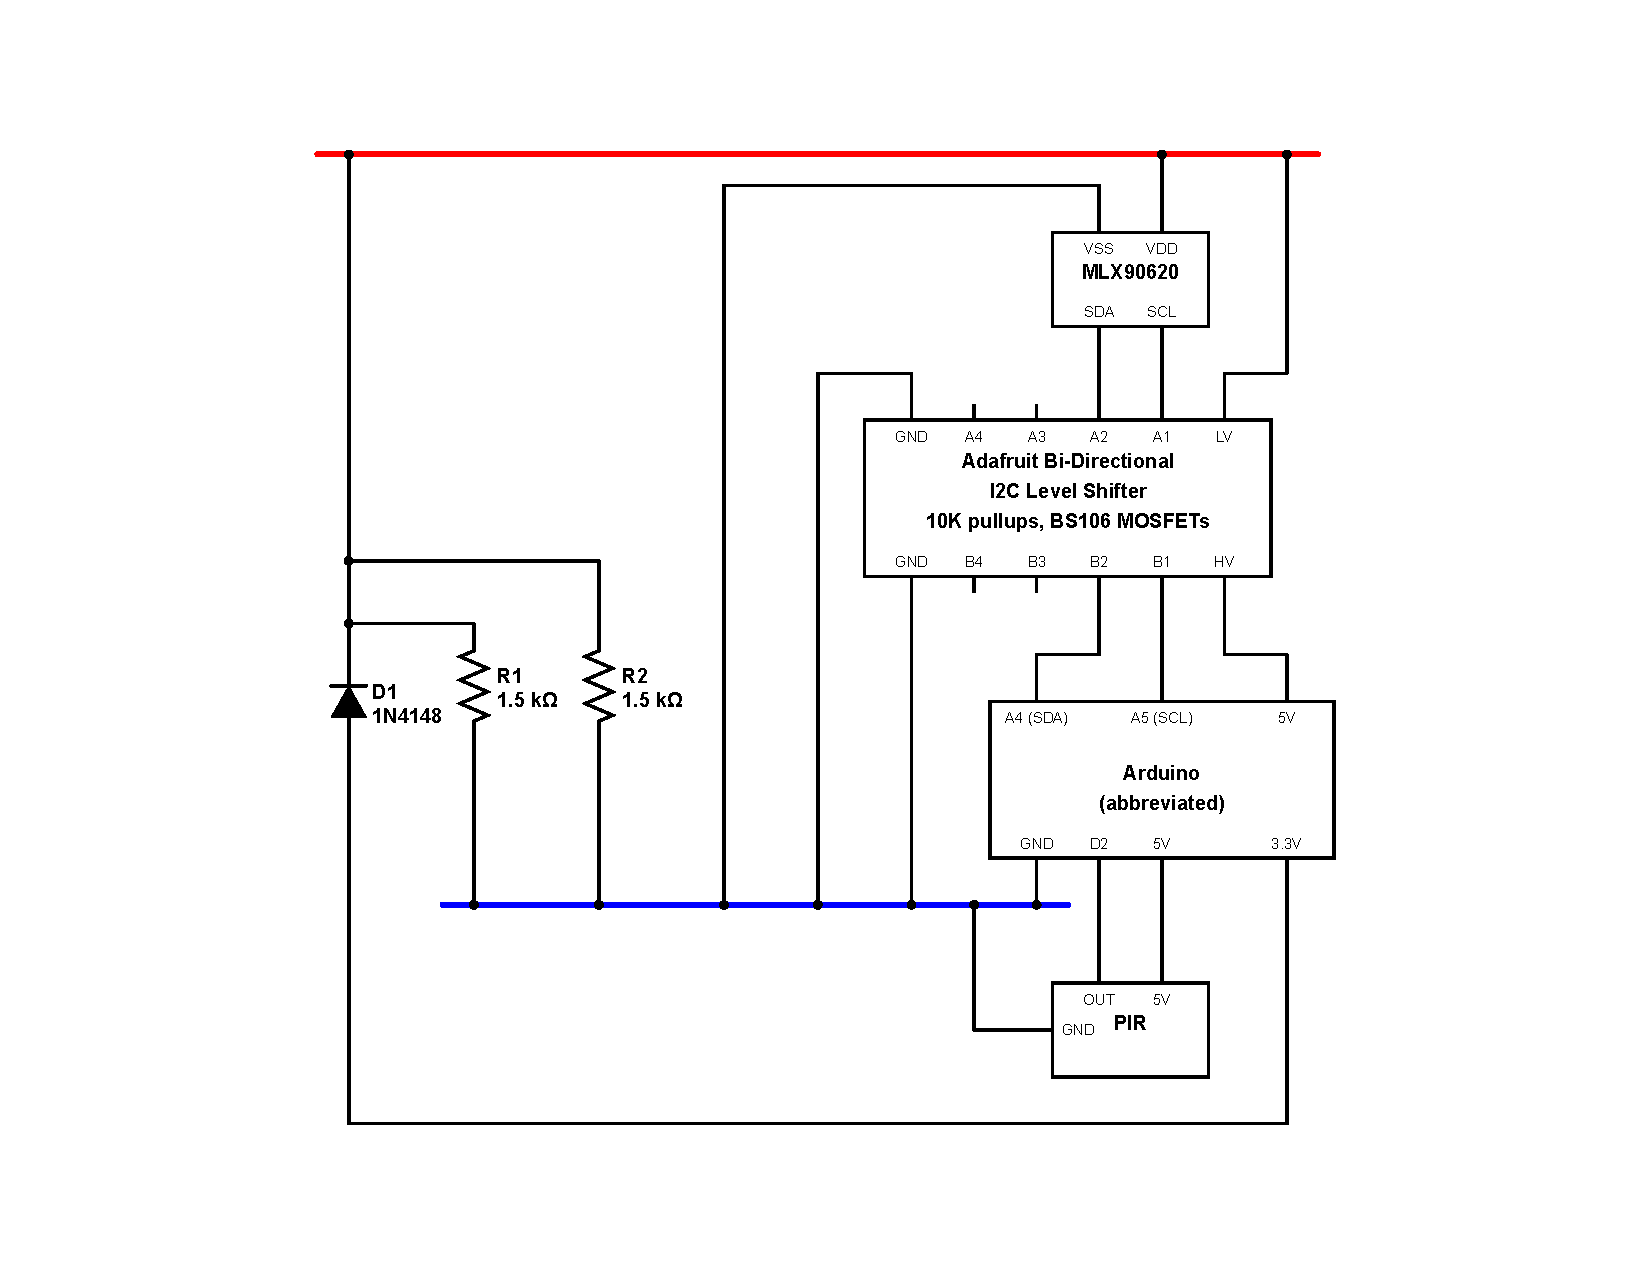
\includegraphics[width=\textwidth]{../diagrams/mlx-arduino.pdf}
\caption{MLX90620, PIR and Arduino integration circuit}
\label{fig:circuits:node}
\end{figure}

Due to low cost and ease of use, the \ard platform was selected as the host for the Preprocessing Tier, and thus the low-level \iic interface for communication to the \mlx. Initially, this presented some challenges, as the \mlx recommends a power and communication voltage of 2.6V, while the \ard is only able to output 3.3V and 5V as power, and 5V as communication. Due to this, it was not possible to directly connect the \ard to the \mlx, and similarly due to the two-way nature of the \iic 2-wire communication protocol, it was also not possible to simply lower the \ard voltage using simple electrical techniques, as such techniques would interfere with two-way communication.

A solution was found in the form of a \iic level-shifter, the Adafruit ``4-channel I2C-safe Bi-directional Logic Level Converter'' \cite{AdafruitI2C}, which provided a cheap method to bi-directionally communicate between the two devices at their own preferred voltages. The layout of the circuit necessary to link the \ard and the \mlx using this converter can be seen in \Fref{fig:circuits:node}.

% TODO: Check PIR settings
Additionally, as used in the Thermosense paper, a \pir motion sensor \cite{AdafruitPIR} was also connected to the \ard. This sensor, operating at 5V natively, did not require any complex circuitry to interface with the \ard. It is connected to digital pin 2 on the \ard, where it provides a rising signal in the event that motion is detected, which can be configured to cause an interrupt on the \ard. In the configuration used in this project, the sensor's sensitivity was set to the highest value and the timeout for re-triggering was set to the lowest value (approximately 2.5 seconds). Additionally, the continuous re-triggering feature (whereby the sensor produces continuous rising and falling signals for the duration of motion) was disabled using the provided jumpers. 

% Talk about RPi and prototype board, and prototype iterations

For the Analysis Tier, the Raspberry Pi B+ was chosen, as it is a powerful computer capable of running Linux available for an extraordinarily low price. The \ard is connected to the Raspberry Pi over USB, which provides it both power and the capacity to transfer data. In turn, the Raspberry Pi is connected to a simple micro-USB rechargeable battery pack, which provides it with power, and subsequently the \ard and sensors.

\section{Software}

To calculate the final temperature values that the \mlx offers, a complex initialisation and computational process must be followed, which is specified in the sensor's datasheet \cite{MLXDatasheet}. This process involves initialising the sensor with values attained from a separate on-board \iic EEPROM, then retrieving a variety of normalisation and adjustment values, along with the raw sensor data, to compute the final temperature result.

The basic algorithm to perform this normalisation was based upon code by users ``maxbot'', ``IIBaboomba'', ``nseidle'' and others on the Arduino Forums \cite{ArduinoForum} and was modified to operate with the newer \ard ``Wire'' \iic libraries released since the authors' posts. In pursuit of the project's aims to create a more approachable thermal sensor, the code was also restructured and rewritten to be both more readable, and to introduce a set of features to make the management of the sensor data easier for the user, and for the information to be more human readable.

The first of the features introduced was the human-readable format for serial transmission. This allows the user to both easily write code that can parse the serial to acquire the serial data, as well as examine the serial data directly with ease. When the \ard first boots running the software, the output in \Fref{fig:code:initseq} is output. This specifies several things that are useful to the user; the attached sensor (``DRIVER''), the build of the software (``BUILD'') and the refresh rate of the sensor (``IRHZ''). Several different headers, such as ``ACTIVE'' and ``INIT'' specify the current millisecond time of the processor, thus indicating how long the execution of the initialisation process took (33 milliseconds).

Once booted, the user is able to send several one-character commands to the sensor to configure operation, which are described in \Fref{tab:ardcommands}. Depending on the sensor configuration, IR data may be periodically output automatically, or otherwise manually triggered. This IR data is produced in the packet format described in \Fref{fig:code:initseq}. This is a simple, human readable format that includes the millisecond time of the processor at the start and end of the calculation, if the \pir has seen any motion for the duration of the calculation, and the 16x4 grid of calculated temperature values.

\begin{figure}
 \centering
\begin{lstlisting}[style=arduino]
INIT 0
INFO START
DRIVER MLX90620
BUILD Feb  1 2015 00:00:00
IRHZ 1
INFO STOP
ACTIVE 33

START 34
MOVEMENT 0
1.0  1.0  1.0  1.0  1.0  1.0  1.0  1.0  1.0  1.0  1.0  1.0  1.0  1.0  1.0  1.0
1.0  1.0  1.0  1.0  1.0  1.0  1.0  1.0  1.0  1.0  1.0  1.0  1.0  1.0  1.0  1.0
1.0  1.0  1.0  1.0  1.0  1.0  1.0  1.0  1.0  1.0  1.0  1.0  1.0  1.0  1.0  1.0
1.0  1.0  1.0  1.0  1.0  1.0  1.0  1.0  1.0  1.0  1.0  1.0  1.0  1.0  1.0  1.0
STOP 97
\end{lstlisting}
\caption{Initialisation sequence and thermal packet}
\label{fig:code:initseq}
\end{figure}

\begin{table}
\centering
\begin{tabular}{|l|l|}
\hline
\texttt{R} & Flush buffers and reset \ard \\ \hline
\texttt{I} & Print INFO again \\ \hline
\texttt{T} & Activate timers for periodic IR data output \\ \hline
\texttt{O} & Deactivate timers for periodic IR data output \\ \hline
\texttt{P} & Manually trigger capture and output of IR data \\ \hline
\texttt{F\textit{x}} & Set sensor refresh frequency to \textit{x} and reboot \\ \hline
\end{tabular}
\caption{Commands}
\label{tab:ardcommands}
\end{table}

\section{Physical Form}
To enable the prototype to be easily mounted on the ceiling, the prototype was placed on a flat board with feet that would enable it to be screwed into a pole, and the pole extended to jam the sensor against the ceiling and the floor using the pole (\Fref{fig:pictures:protob1}, \Fref{fig:pictures:protoact}). Due to a wireless module and battery pack being added to the Raspberry Pi, it was feasible for the sensor to operate entirely wirelessly for several hours. However, in most cases it was more convenient to operate using wired power and Ethernet.

\begin{figure}
\centering
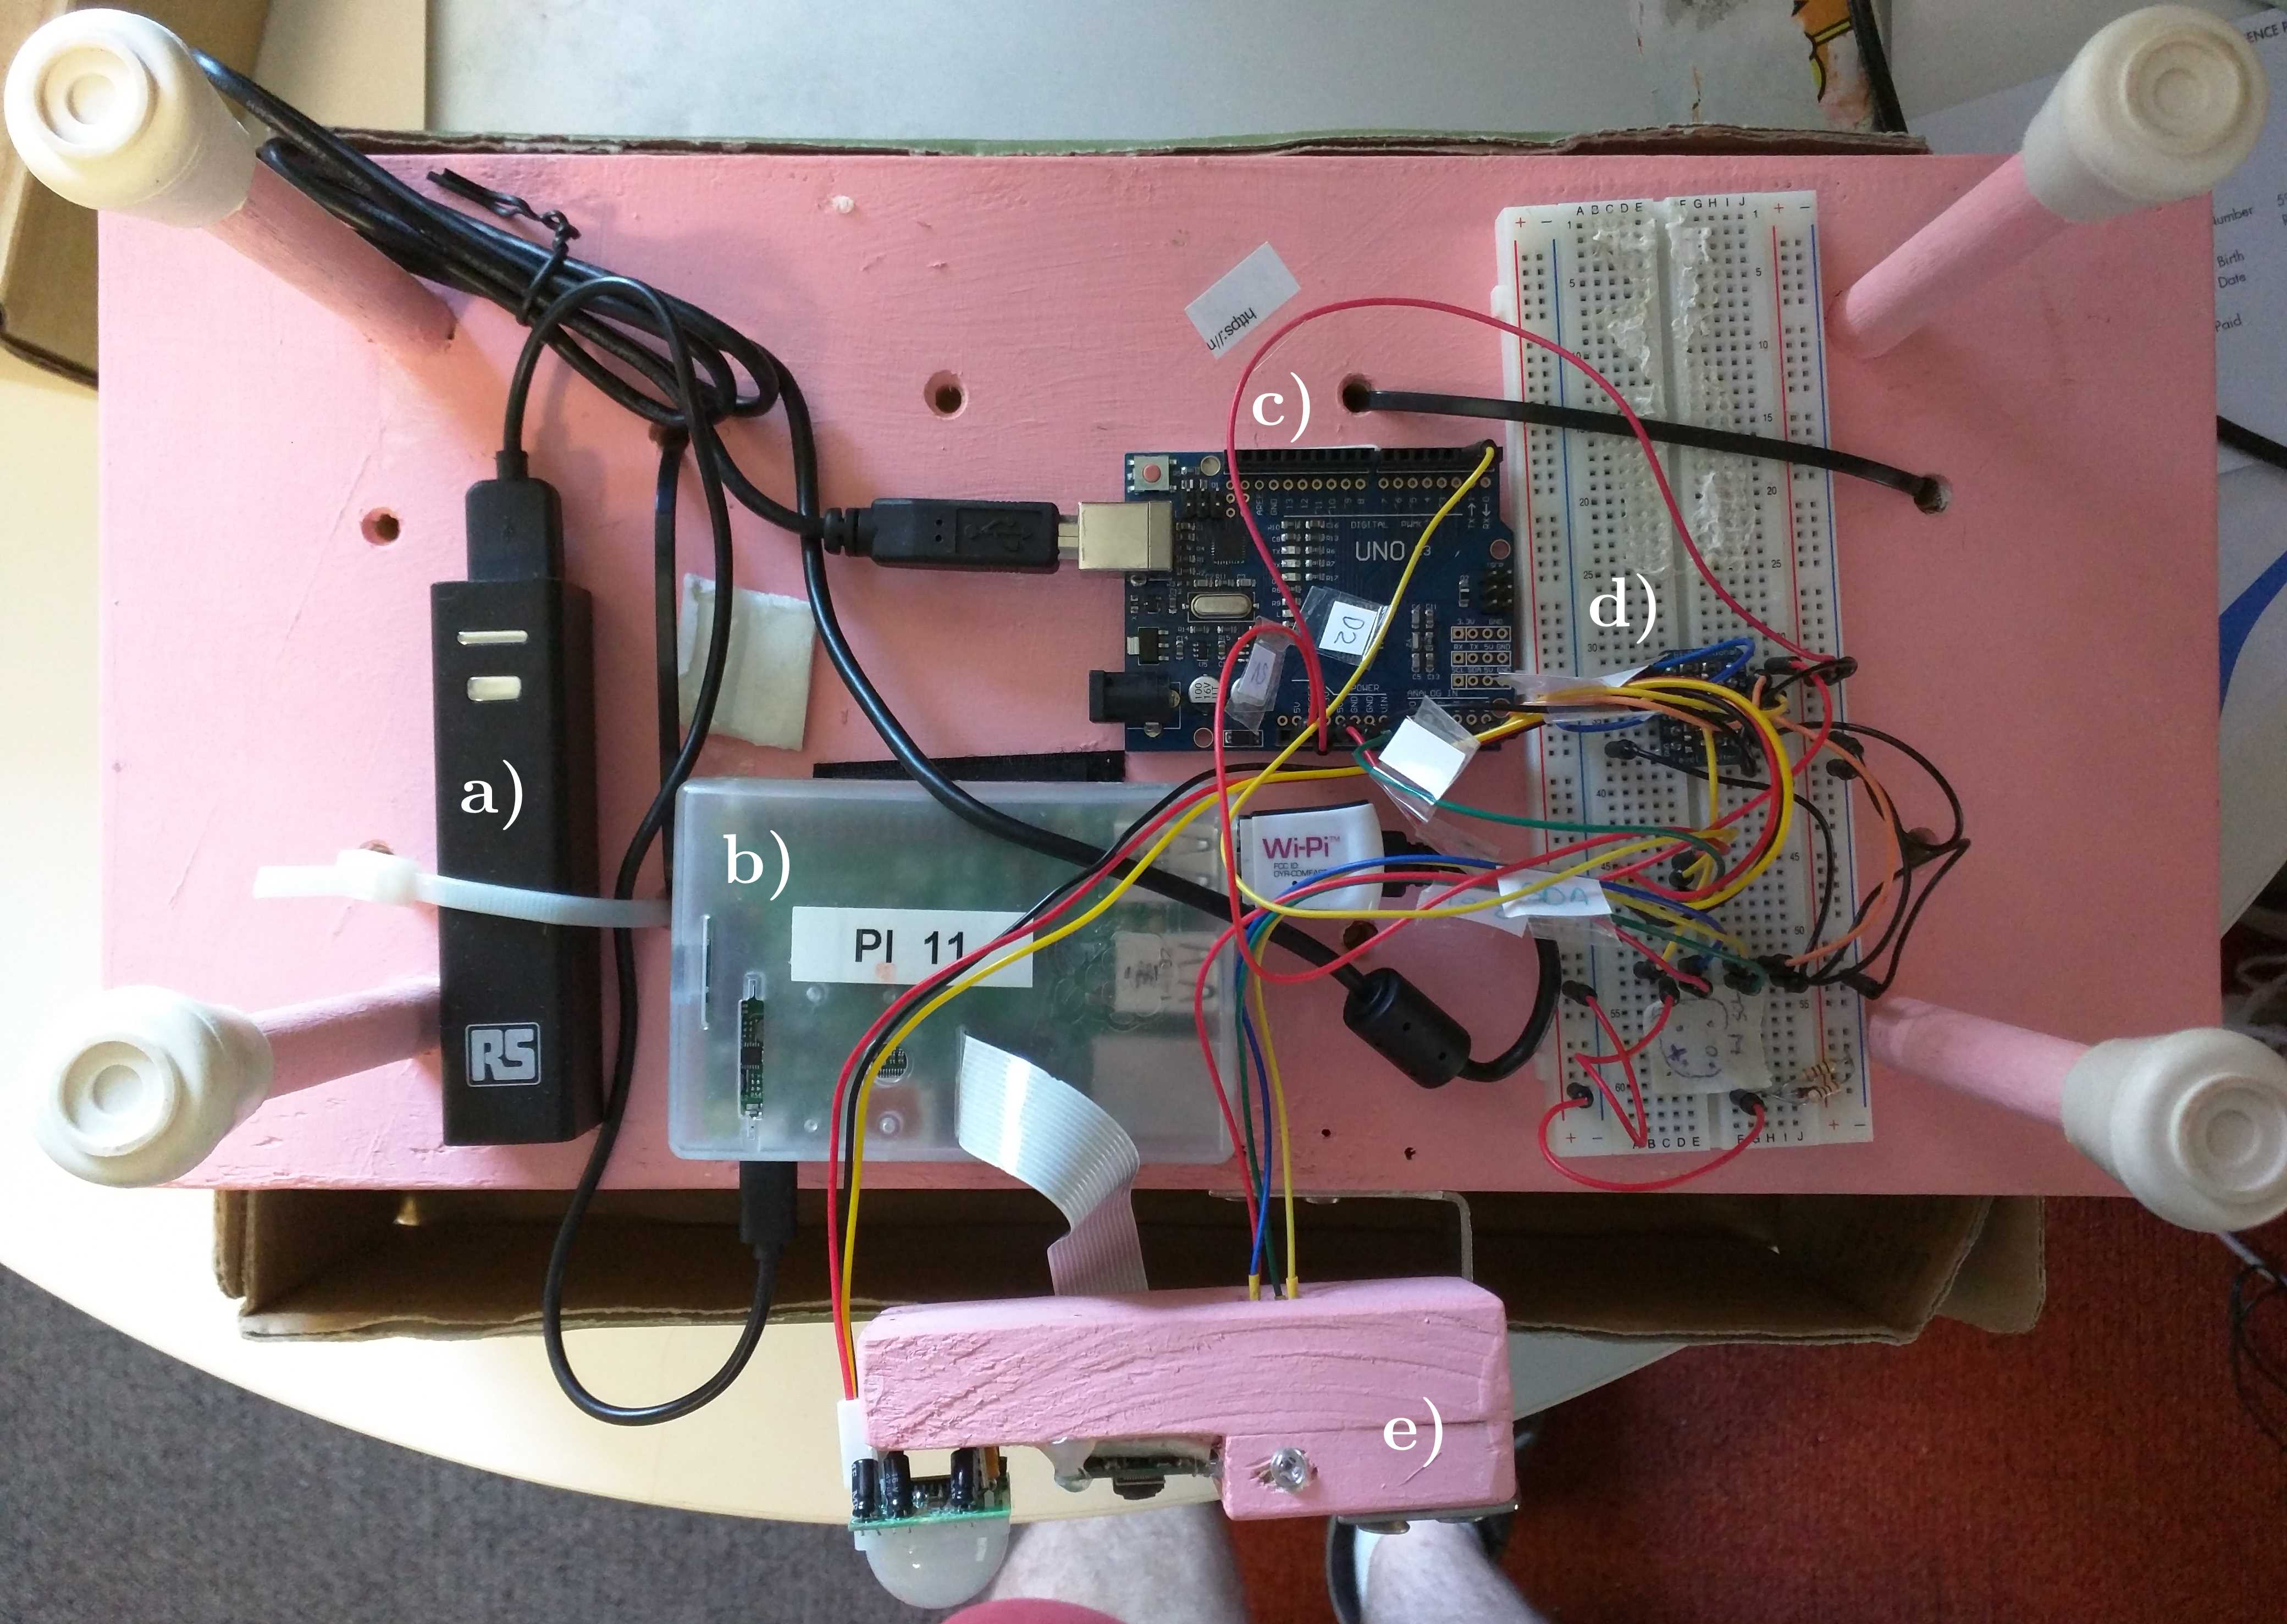
\includegraphics[width=\textwidth]{../diagrams/prototypeb-1.jpg}
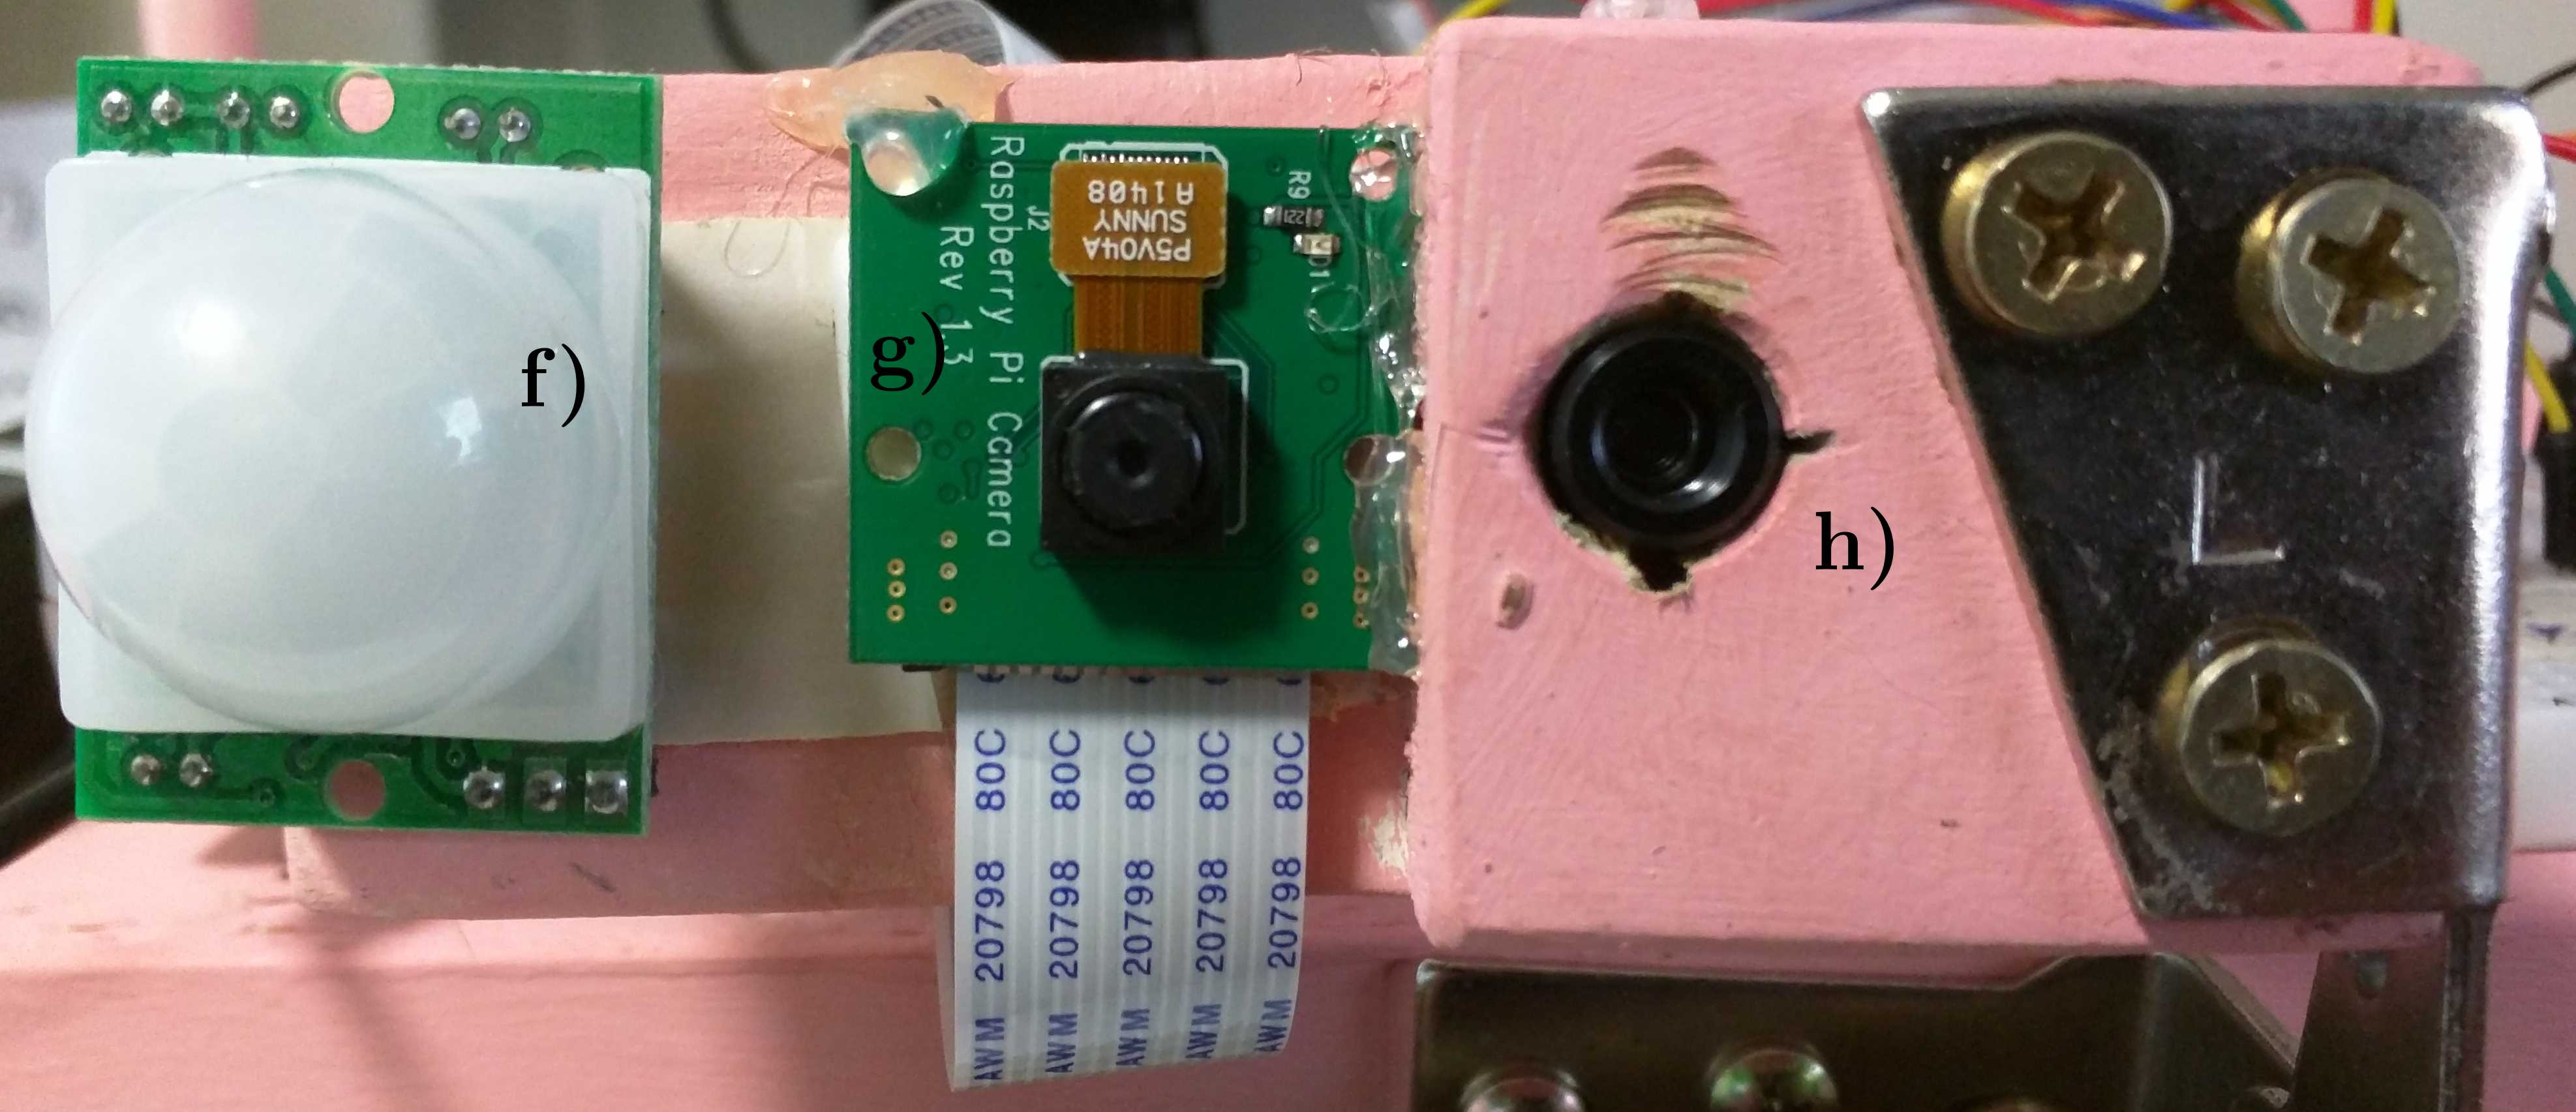
\includegraphics[width=\textwidth]{../diagrams/prototypeb-2.jpg}
{\small
\begin{multicols}{2}
\begin{enumerate}[a)]
 \item Battery pack
 \item Raspberry Pi
 \item Arduino
 \item Level-shifting circuitry
 \item Movable sensor mount
 \item PIR
 \item Camera
 \item \mlx
\end{enumerate}
\end{multicols}
}
\caption{Prototype Physical Form}
\label{fig:pictures:protob1}
\end{figure}

\begin{figure}
\centering
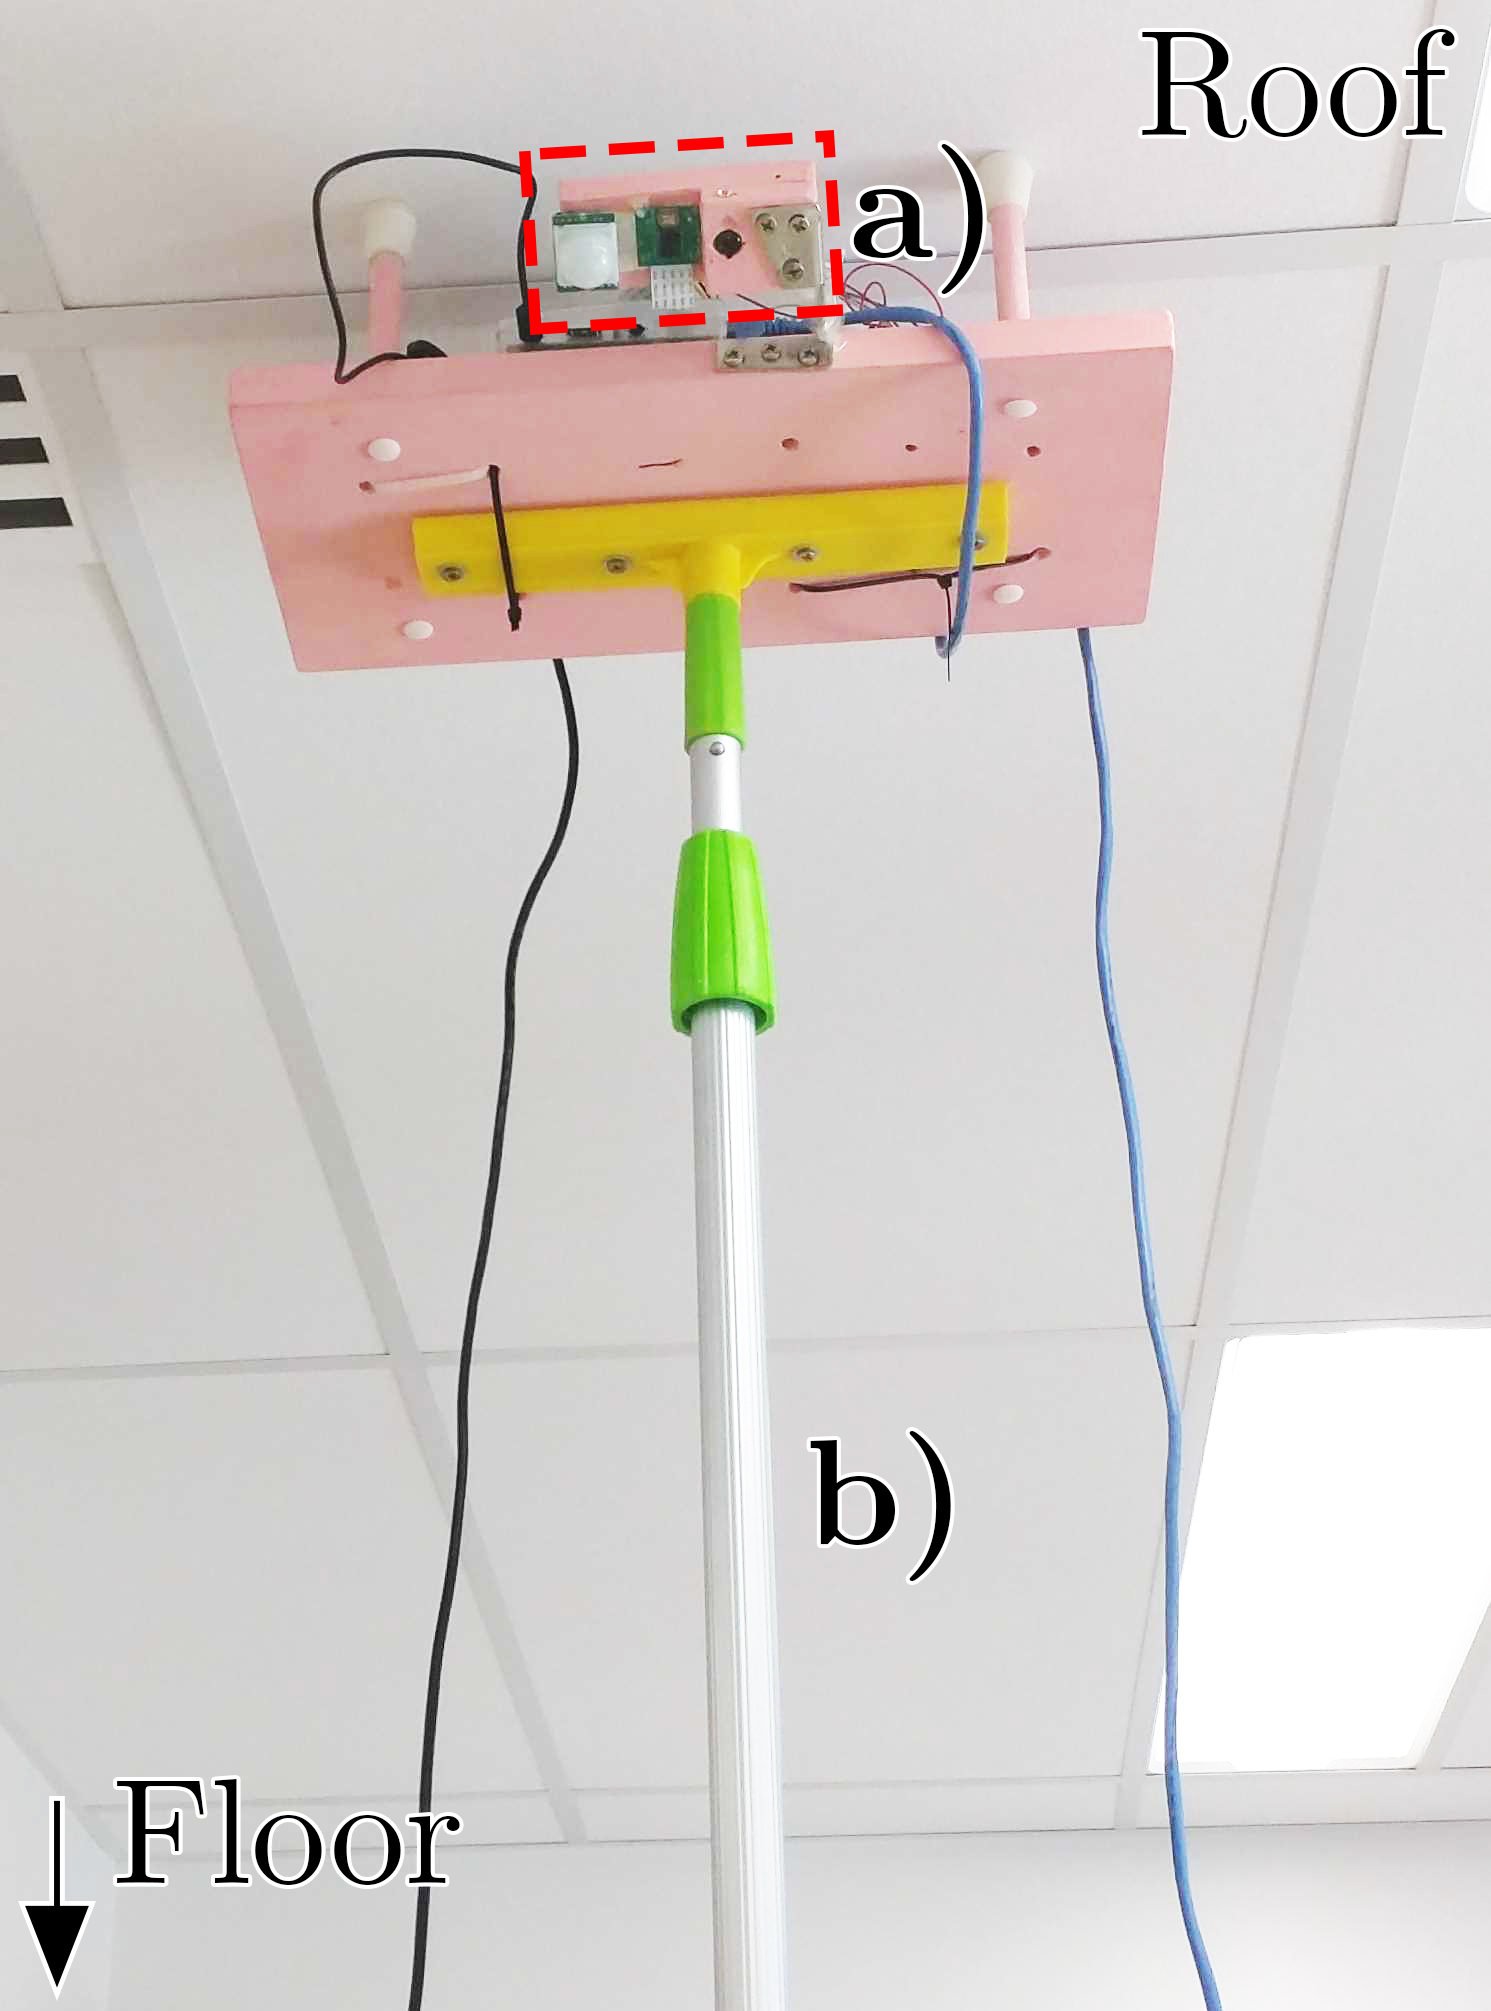
\includegraphics[height=0.5\textheight]{../diagrams/prototype-mounted-ceiling.jpg}
\caption{Prototype in action}
\label{fig:pictures:protoact}
\end{figure}

\begin{figure}
\centering
\begin{tikzpicture}[node distance=1.7cm]
\node (interwebs) [cbox] {Network};
\node (wifi) [dashbox, right=of interwebs] {\small WiFi / Ethernet};
\node (rpi) [fcont, below=of wifi] {Raspberry Pi \linebreak
  ``Analysis Tier'' \linebreak
  
  \tikz\node[fbox, minimum width=2.3cm, text width=2.3cm] {\small \ttfamily thinglib};
  \tikz\node[fbox, minimum width=2.3cm, text width=2.3cm] {\small \ttfamily features.py};
};
\node (cam) [box, right=of rpi] {Camera};
\node (usb) [dashbox, below=of rpi] {\small USB Serial};
\node (ard) [fcont, below=of usb] {Arduino \linebreak
  ``Preprocessing Tier'' \linebreak
  
  \tikz\node[fbox, minimum width=3.3cm, text width=3.3cm] {\small \ttfamily mlx90620\_driver};
};
\node (iic) [dashbox, left=of ard] {\small \iic};
\node (mlx) [box, below=of iic] {MLX90620};
\node (wire) [dashbox, right=of ard] {\small Interrupt};
\node (pir) [box, below=of wire] {PIR};
\node (sensetier) [dashbox, dotted, fit=(pir) (mlx)] {``Sensing Tier''};

\draw [line] (interwebs) -- (wifi);
\draw [line] (wifi) -- (rpi);
\draw [line] (rpi) -- (usb);
\draw [line] (usb) -- (ard);
\draw [line] (ard) -- (iic);
\draw [line] (iic) -- (mlx);
\draw [line] (ard) -- (wire);
\draw [line] (wire) -- (pir);
\draw [line] (rpi) -- (cam);
\end{tikzpicture}
\caption{Prototype system architecture}
\label{fig:pictures:protob-arch}
\end{figure}


\section{Sensor Properties}
See \Fref{fig:exps:2setup}.

\begin{figure}
\centering
% TODO: Need proper figure merging
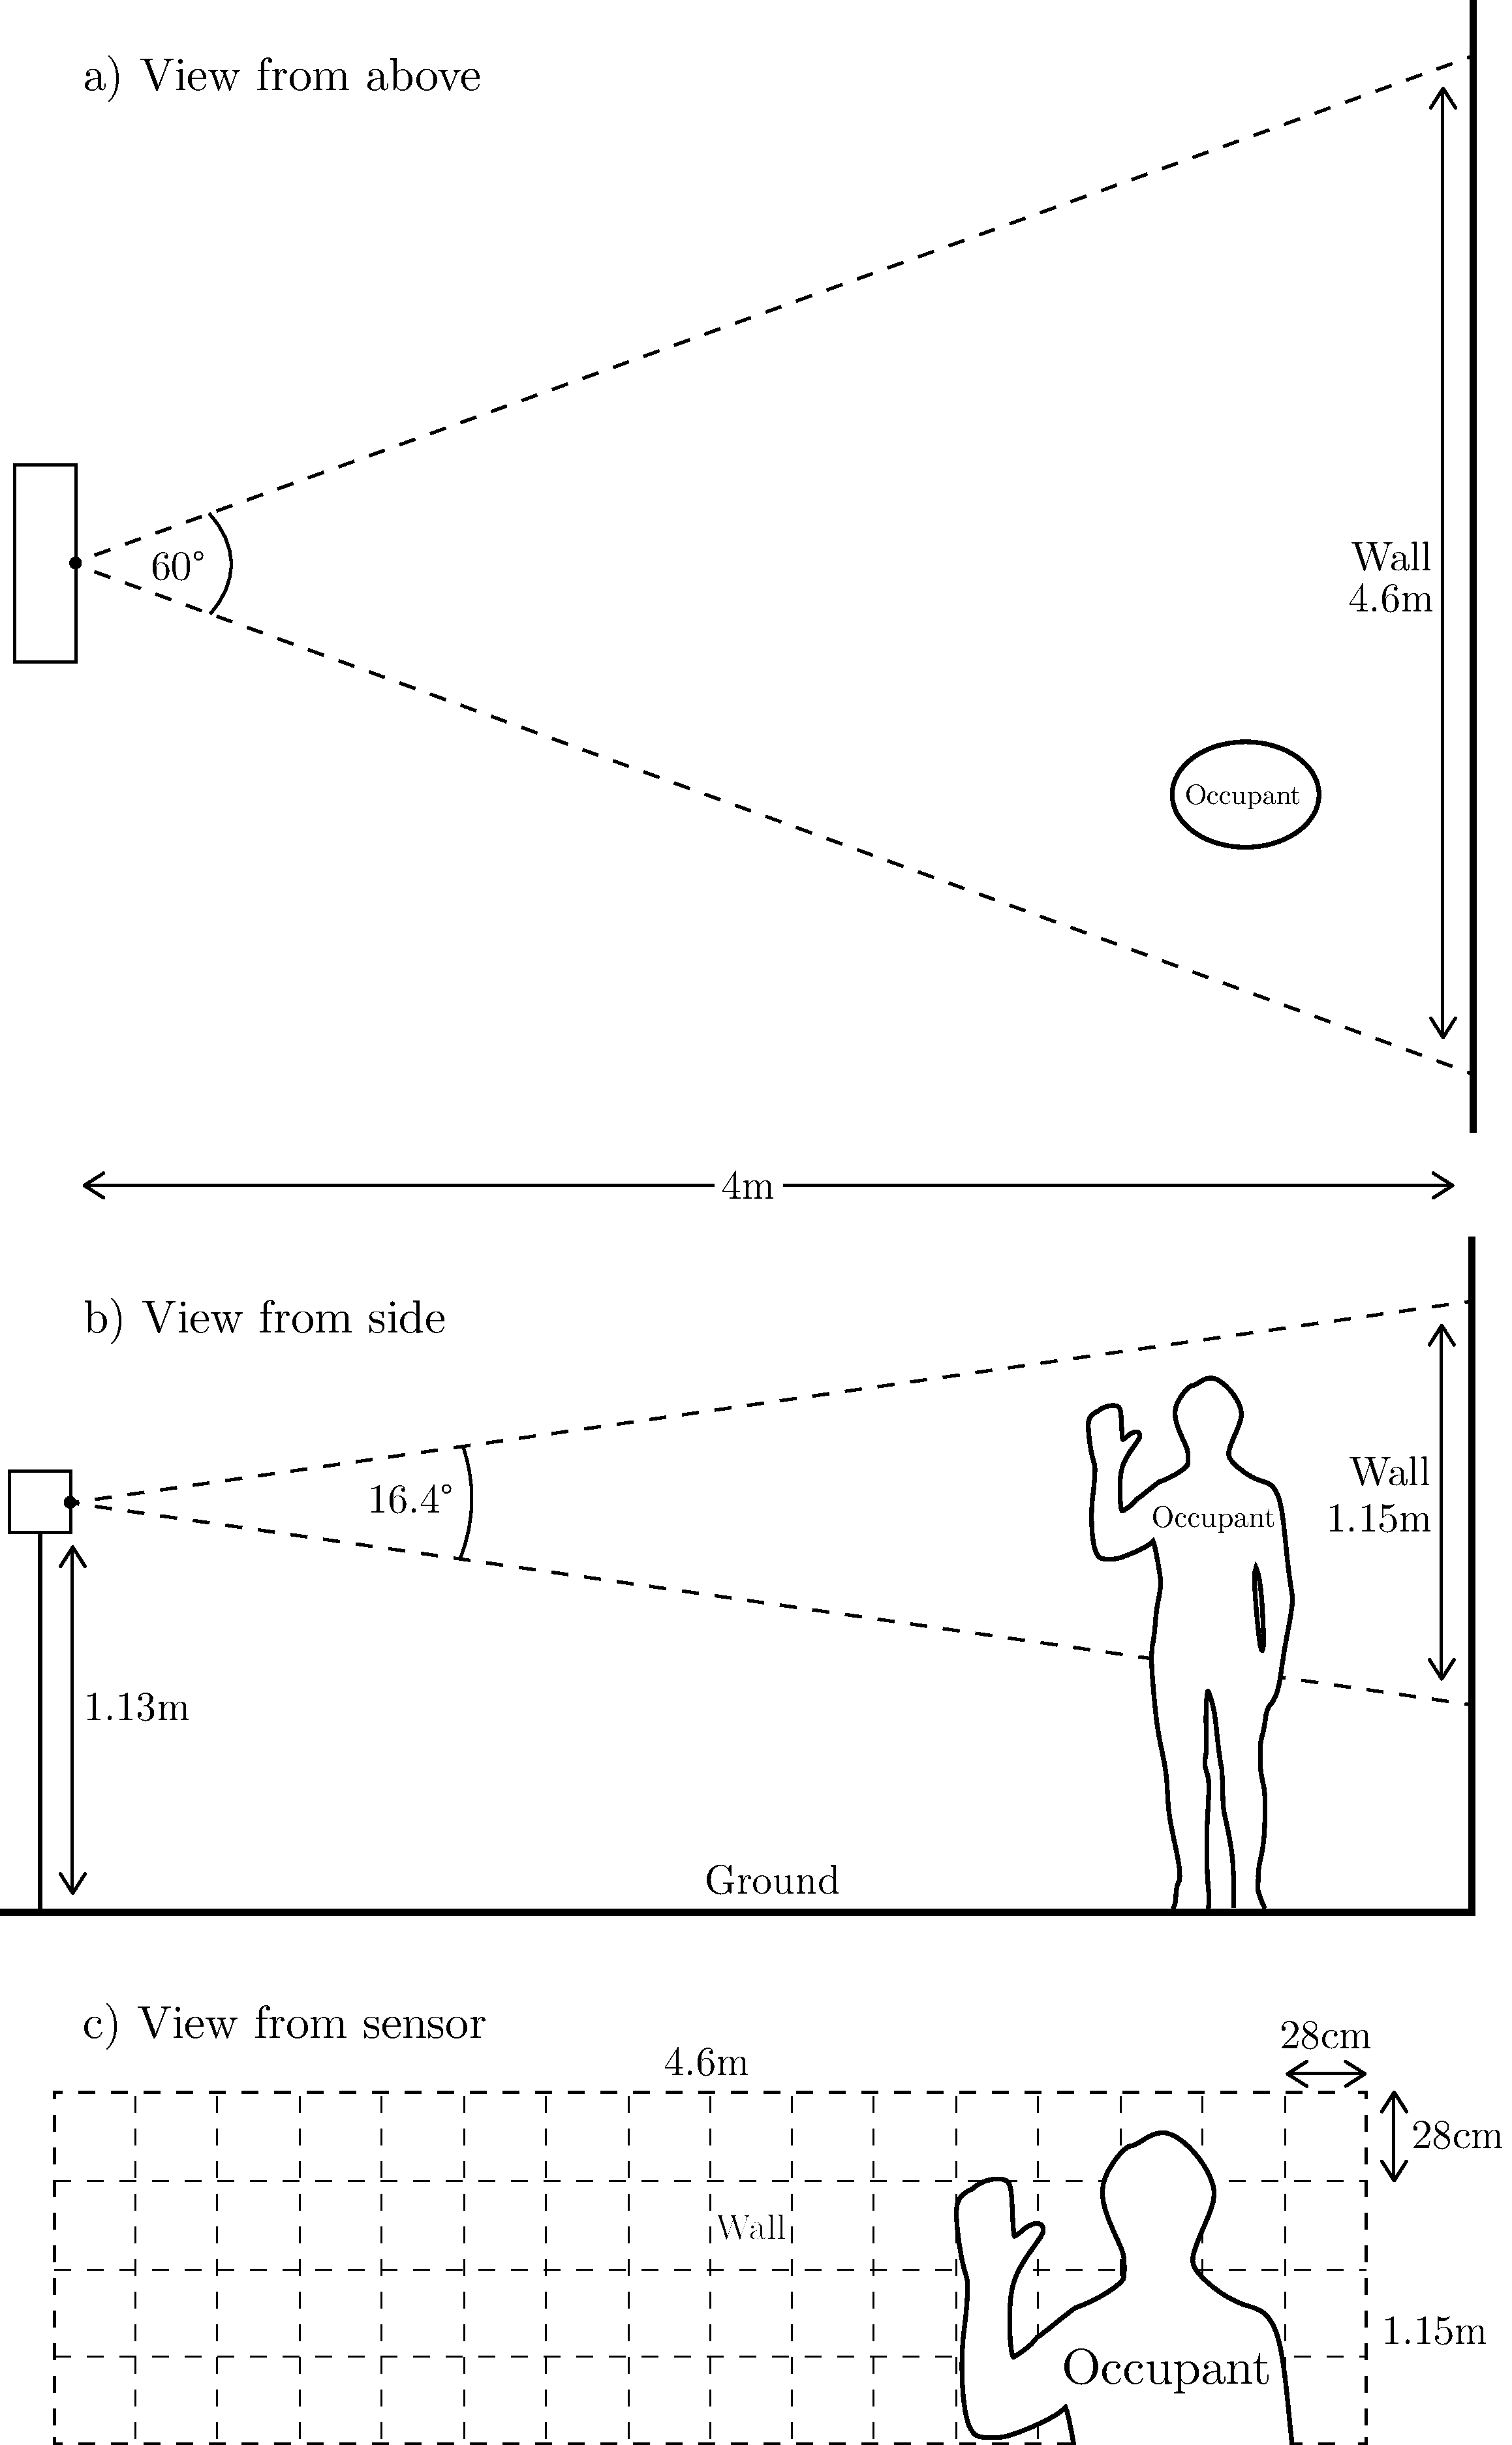
\includegraphics[height=0.9\textheight]{../diagrams/second-exp-setup2.pdf}
\caption{Experiment setup to determine sensor properties}
\label{fig:exps:2setup}
\end{figure}

%\afterpage{\global\pdfpageattr\expandafter{\the\pdfpageattr/Rotate 90}}
\begin{sidewaystable}
{\small
\begin{tabular}{*{16}{|z{2.5em}}|}
\hline
14.95 0.51 & 14.33 0.27 & 12.34 0.27 & 8.77 0.33 & 8.15 0.31 & 10.84 0.38 & 9.02 0.26 & 7.79 0.37 & 6.67 0.27 & 9.63 0.29 & 9.29 0.26 & 8.24 0.27 & 9.84 0.25 & 14.28 0.33 & 14.92 0.3 & 13.16 0.25 \\ \hline
14.54 0.34 & 15.62 0.31 & 12.73 0.23 & 11.51 0.27 & 11.79 0.26 & 11.47 0.27 & 11.43 0.29 & 9.02 0.35 & 8.57 0.23 & 11.15 0.23 & 10.64 0.22 & 10.3 0.24 & 12.09 0.22 & 14.49 0.26 & 14.88 0.31 & 14.71 0.36 \\ \hline
18.25 0.45 & 16.62 0.31 & 14.15 0.24 & 11.97 0.34 & 13.11 0.3 & 12.64 0.22 & 10.66 0.23 & 9.15 0.24 & 9.58 0.28 & 11.95 0.28 & 11.22 0.24 & 11.52 0.36 & 11.11 0.23 & 12.59 0.25 & 14.44 0.31 & 13.35 0.28 \\ \hline
16.02 0.28 & 16.81 0.36 & 15.0 0.25 & 11.53 0.28 & 10.18 0.29 & 12.2 0.25 & 11.78 0.29 & 8.36 0.31 & 8.15 0.33 & 10.36 0.32 & 10.74 0.31 & 8.25 0.36 & 9.99 0.35 & 12.42 0.38 & 11.39 0.4 & 11.06 0.34 \\ \hline
\end{tabular}
}
\caption{Mean and standard deviations for each pixel at rest}
\label{tab:meanstd}
\end{sidewaystable}
%\afterpage{\global\pdfpageattr\expandafter{\the\pdfpageattr/Rotate 0}}

In \Fref{tab:meanstd} the thermal sensor was exposed to the night sky at a capture rate of 1Hz for 4 minutes, with the sensing results combined to create a set of means and standard deviations to indicate the pixels at ``rest''.


\begin{figure}
\centering
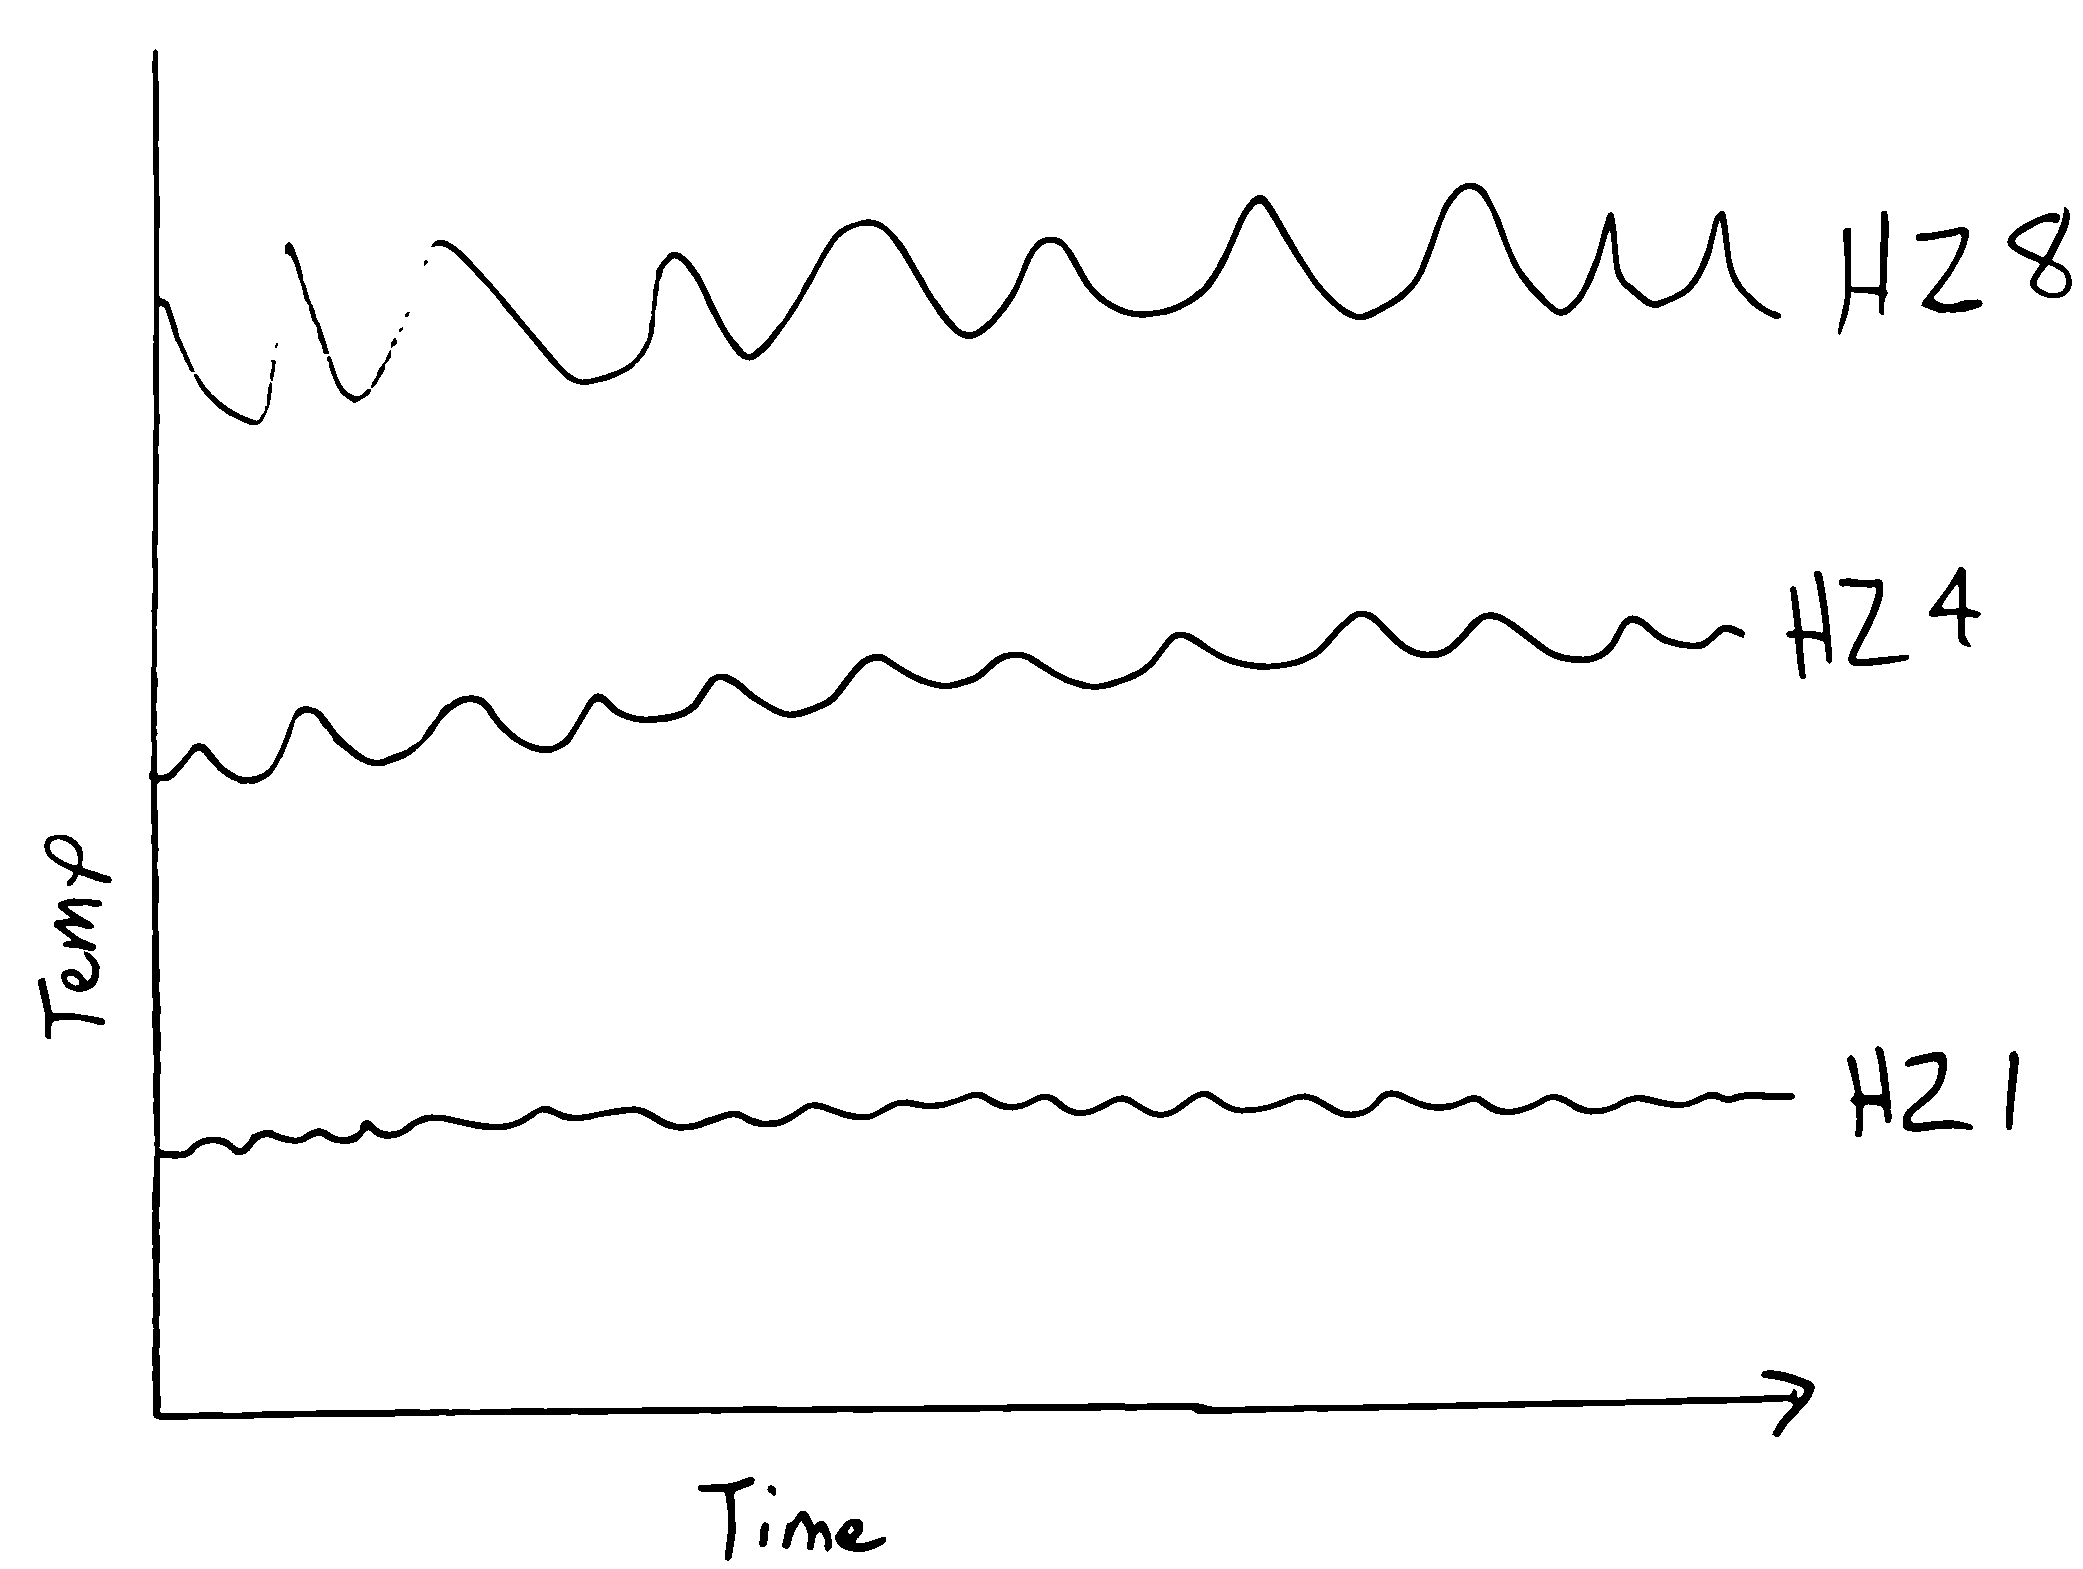
\includegraphics[width=\textwidth]{../diagrams/temp/noise.pdf}
\caption{Comparison of noise levels at the \mlx' various sampling speeds}
\label{fig:noise}
\end{figure}

\begin{figure}
\centering
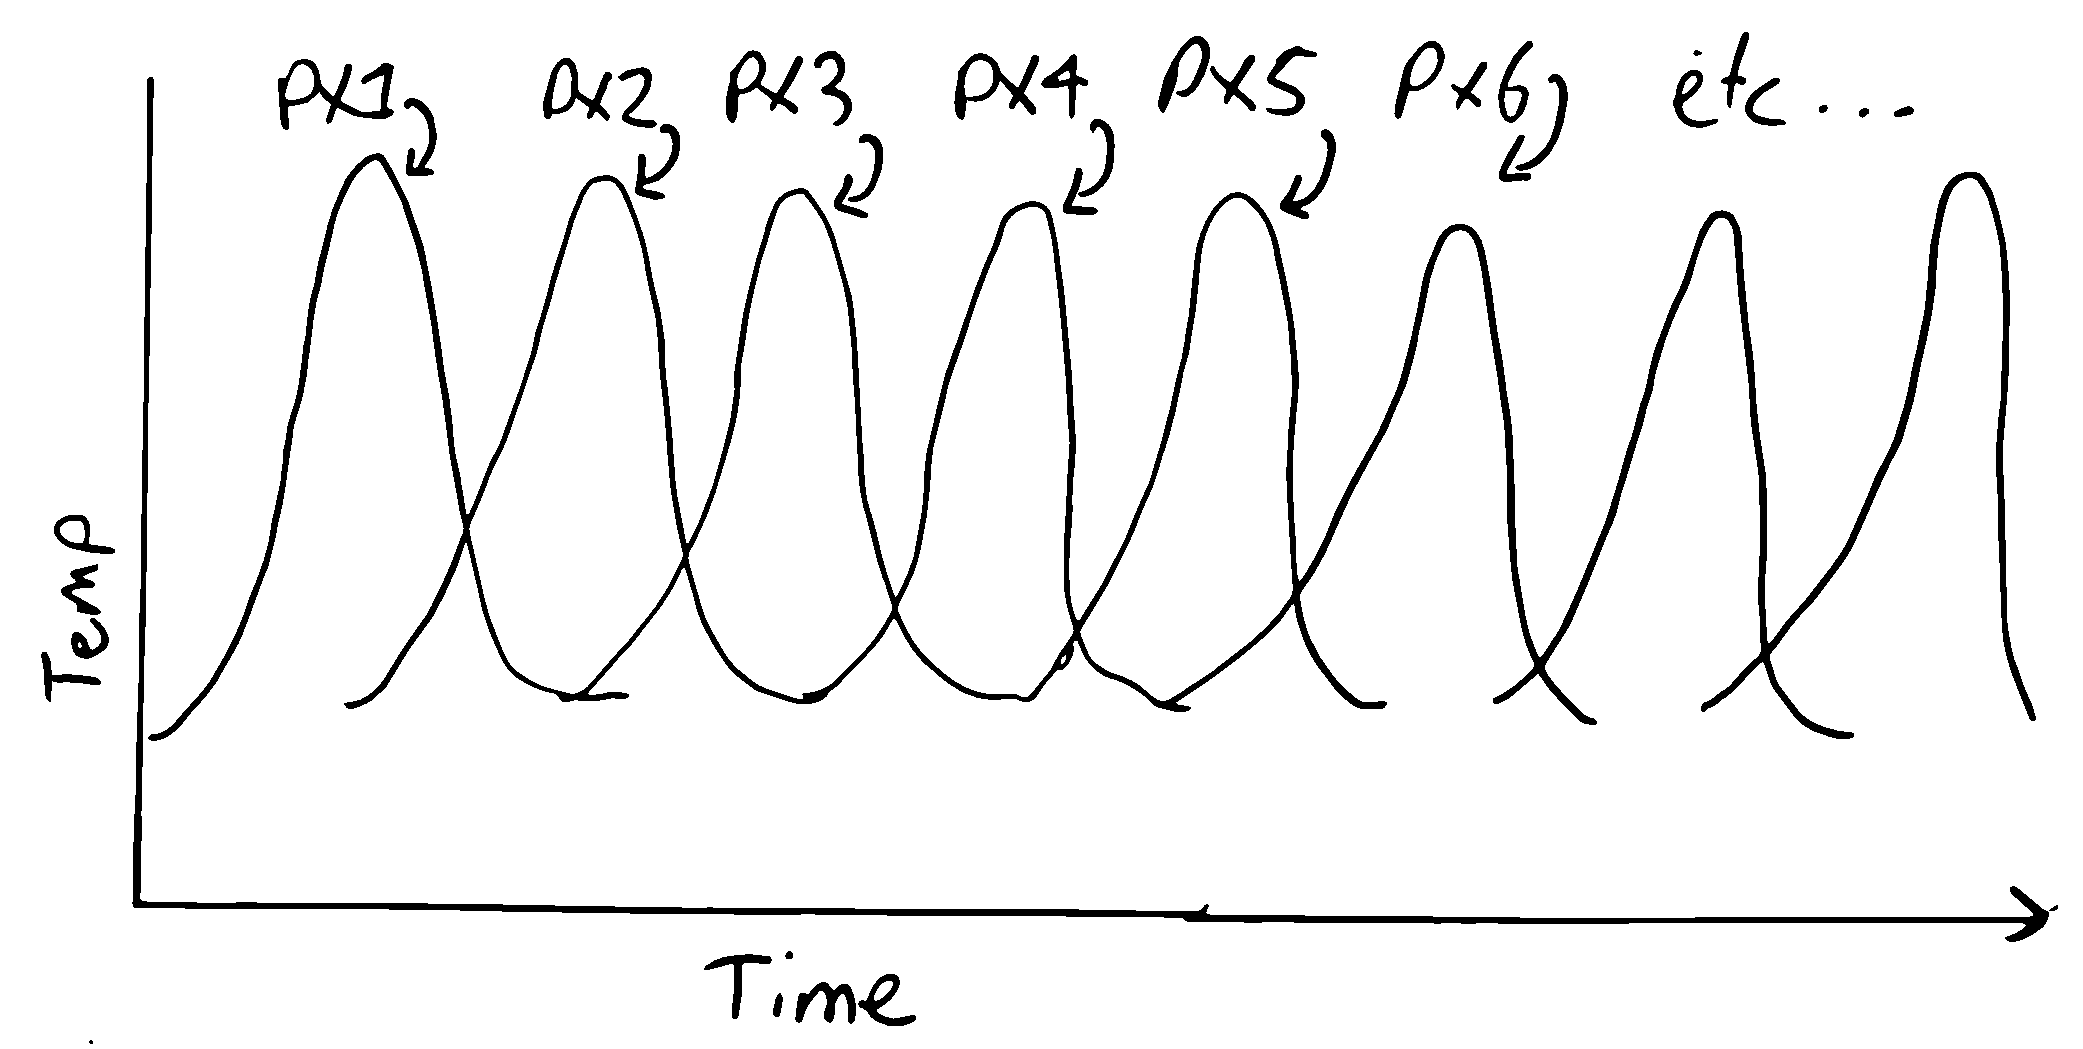
\includegraphics[width=\textwidth]{../diagrams/temp/motion.pdf}
\caption{Different \mlx pixel temperature values as hot object moves across row}
\label{fig:hotmotion}
\end{figure}

\begin{figure}
\centering
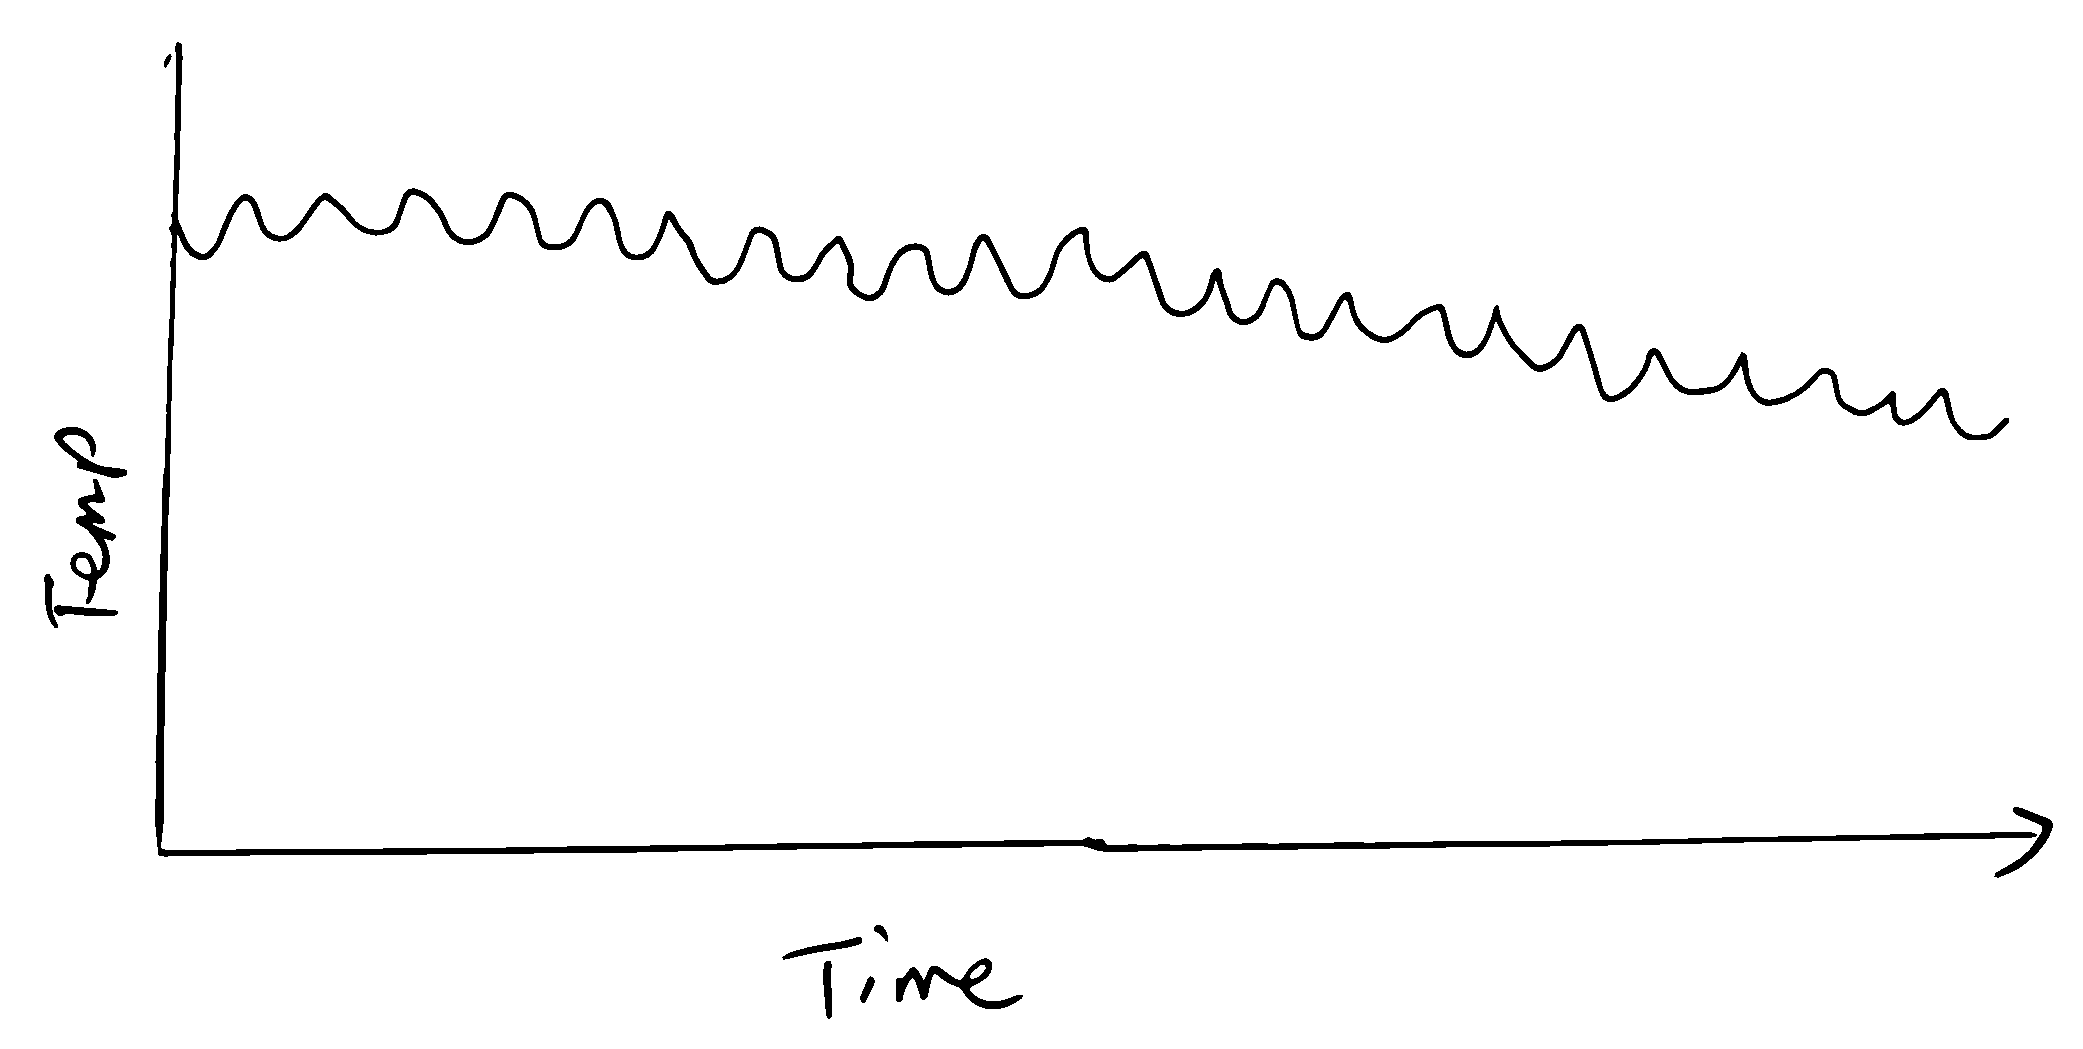
\includegraphics[width=\textwidth]{../diagrams/temp/cooldown.pdf}
\caption{Variation in temperature detected for hot object at 1Hz sampling ration}
\label{fig:cooldown}
\end{figure}
 
 \ifcsdef{mainfile}{}{\bibliography{../references/primary}}
\end{document}
